%%%%%%%%%%%%%%%%%%%%%%%%%%%%%%%%%%%%%%%%%%%%%%%%%%%%%%%%%%%%%%%%%%%
%%% Documento LaTeX 																						%%%
%%%%%%%%%%%%%%%%%%%%%%%%%%%%%%%%%%%%%%%%%%%%%%%%%%%%%%%%%%%%%%%%%%%
% Título:		Capítulo 3
% Autor:  	Ignacio Moreno Doblas
% Fecha:  	2014-02-01, actualizado 2019-11-11
% Versión:	0.5.0
%%%%%%%%%%%%%%%%%%%%%%%%%%%%%%%%%%%%%%%%%%%%%%%%%%%%%%%%%%%%%%%%%%%
% !TEX root = A0.MiTFG.tex

\section{Iteración inicial: Planteamiento básico}
        \subsection{Resumen}
        
        Esta primera iteración consiste en la selección justificada del hardware y software en los que se basará todo el proyecto.
        
        \subsection{Desarrollo}

        El proyecto consta de dos partes fundamentales. Primeramente un panel de control desde el cual un usuario podrá modificar los datos de entrada y observar los resultados del análisis de efectividad y eficiencia de los algoritmos. En segundo lugar debe existir un dispositivo el cual lleve a cabo las evaluaciones de los algoritmos de tiempo real.

        Para el panel de control se ha decidido emplear QT 4.9.0 gracias al cual se evita tener que gestionar los componentes gráficos de la interfaz, pudiendo centrar el esfuerzo mayoritariamente en el tratamiento de los datos y las interacciones de usuario.
        
        Para el hardware del dispositivo en tiempo real se ha escogido una Tiva C Series (TM4C123GXL) por sus numerosos modos de bajo consumo y familiaridad con el dispositivo.        

        \subsection{Diagramas}

        Una vez especificados el hardware y software a emplear se vuelve posible, y necesario, profundizar en los diagramas realizados anteriormente añadiendo cuestiones ya específicas de la solución escogida para el desarrollo del proyecto. Teniendo en cuenta las características de la tecnología escogida se ha realizado el diagrama \ref{fig:InternalBlocksDiagram}, detallando el flujo de trabajo del proyecto.

        \begin{figure}[H]  
            \centering
                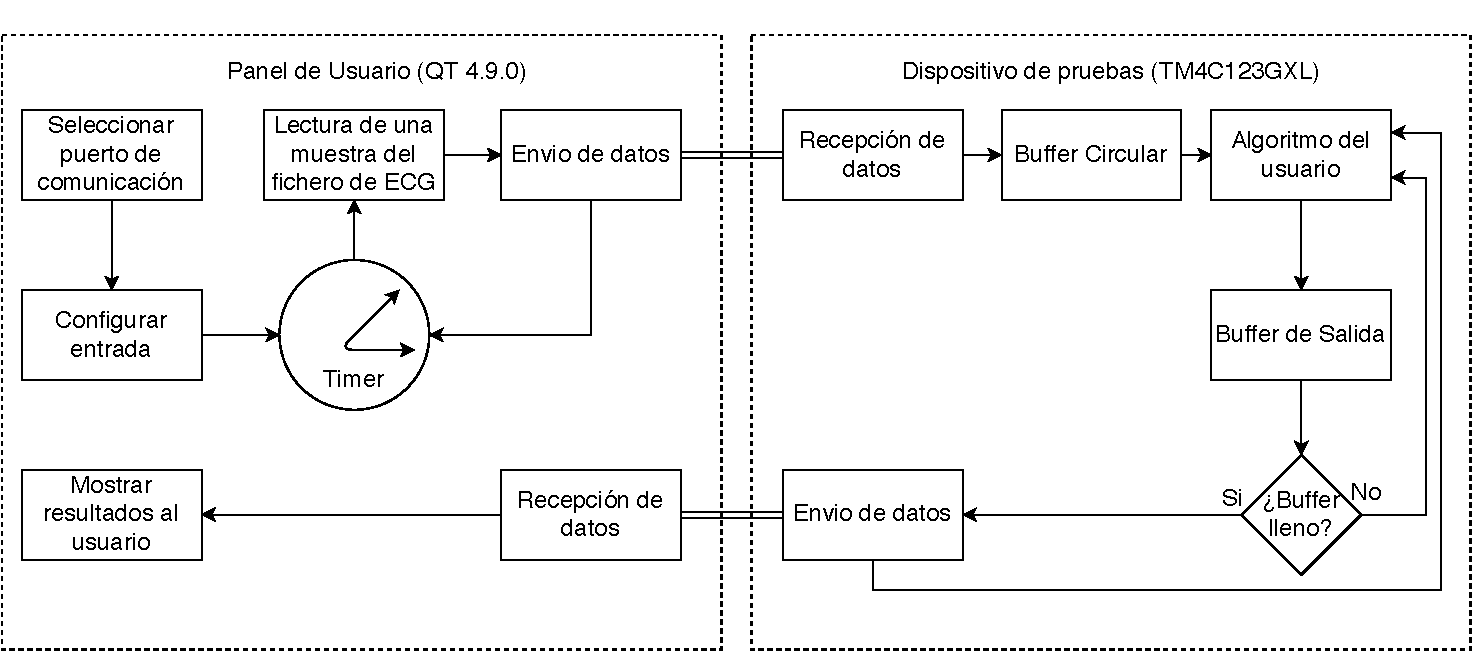
\includegraphics[width =\linewidth]{figuras/InternBlockDiagram.pdf}
                \caption{Diagrama de bloques general}
                \label{fig:InternalBlocksDiagram}
        \end{figure}
 
        La parte izquierda de la figura \ref{fig:InternalBlocksDiagram} representa la funcionalidad mínima necesaria para el panel de control y la parte derecha el flujo de trabajo del hardware de testeo. En un comienzo el factor “Tiempo Real” vendrá determinado por un timer en el panel de control que enviará muestras del ECG de forma cíclica a la frecuencia de muestreo que este se encuentre registrado, simulando así los tiempos biológicos reales de dichas señales. 
        
        Los datos son almacenados en un buffer circular, el cual una vez lleno comenzará a sobrescribir los datos más antiguos. El algoritmo introducido deberá emplear únicamente los datos almacenados en el buffer circular para llevar a cabo el análisis. Como en la vuelta de los datos no es tan importante simular el tiempo real se ha decidido devolverlos al panel en forma de paquetes, saturando menos la vía de comunicaciones.
        
        Una vez devuelta la información al panel de control este deberá mostrar de alguna forma los datos al usuario que lo controla.        

        \subsection{Conclusiones}

        Decidida la estructura general del proyecto, puede comenzar la primera iteración de desarrollo, en la que se implementará la funcionalidad básica, sentando las bases para todo el desarrollo posterior.